%This is a LaTeX template for homework assignments
\documentclass{article}

\usepackage[utf8]{inputenc}
\usepackage{amsmath}
\usepackage{amssymb}
\usepackage{graphicx}
\usepackage{enumitem}
\usepackage{multirow}
\usepackage{minted}

\usepackage[a4paper, margin=1in]{geometry}

\begin{document}

%\title{EMET1001: ASSIGNMENT WEEK 2}
%\author{ZEMING WANG - U6114134}


%\maketitle
%\vspace{1in}

%TUTOR: LONG

\thispagestyle{empty}

\begin{center}
\huge
\vspace*{2.0in} EMET8005 
\\\vspace{0.5in} ASSIGNMENT 1
\normalsize
\\\vspace{0.5in} \textsc{By}
\\\vspace{0.1in} \textsc{Zeming Wang}
\\\vspace{0.1in} \textsc{u6114134}
\normalsize
\\\vspace{0.5in} \textsc{Lecturer: Tue Gørgens}
\\\vspace{0.1in} \textsc{Tutor: Luis Uzeda Garcia}
\normalsize
\\\vspace{0.5in} \textsc{Due: Mar. 30, 2017}
\end{center}

\newpage
\setcounter{page}{1}

\subsection*{A mob of kangaroos}
\begin{enumerate}
    \item[(a)] The regression with only height and age shows that there is a negative relationship between the two, while the regression with height, age and gender shows that there is a positive relationship between height and age and a negative relationship between height and gender. \\
    
    This is probably because the negative relationship observed in the former regression model is actually due to the gender factor, i.e. female kangaroos are generally live longer but shorter in height. The later regression model show that, there is indeed a negative relationship between gender and height, and if the gender issue is factored out, height should increase as age increases. \\
    
    \item[(b)] To verity the interpretation in (a), plot the height and age data in a scatter graph with respect to male and female separately, and run regressions on each separately. The graph is as below:\\
    
    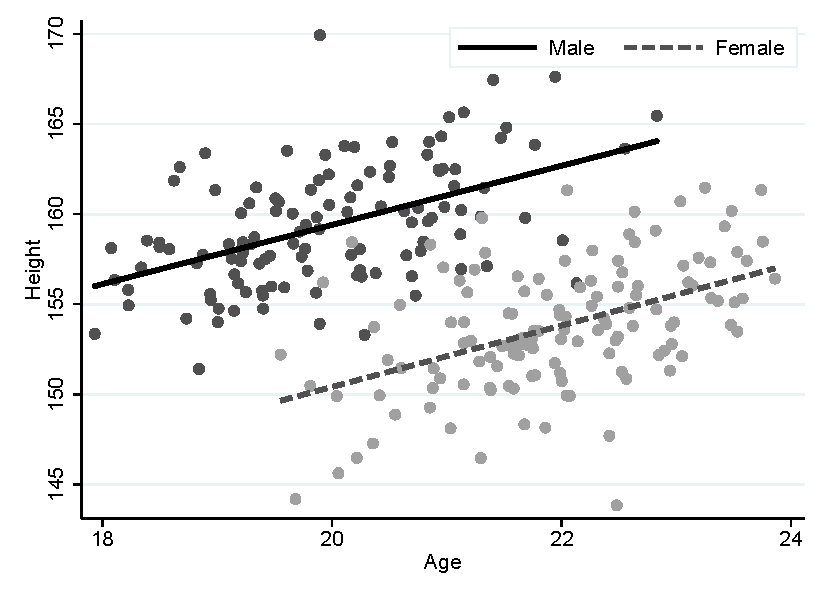
\includegraphics{Graph1}
    
    As we can see clearly in the graph, female kangaroos generally live longer, but male kangaroos are generally taller and within male or female group only, the height grows as age increases, which verifies our speculation in part (a). \\
    
\end{enumerate}


\subsection*{Colombian private school vouchers}
\begin{enumerate}
    \item[(a)] The numbers of students who attempted and completed the interview are counted as below (records without lottery outcome are skipped): 
        \begin{minted}{text}
        -----------+---------------------------------
         Attempted |       Completed interview
         interview |         0          1       Total
        -----------+----------------------+----------
                 0 |     1,795          0 |     1,795 
                 1 |     1,073      1,176 |     2,249 
        -----------+----------------------+----------
             Total |     2,868      1,176 |     4,044
        -----------+---------------------------------
        \end{minted}
    
    There are total 4044 valid records, 2248 attempted and 1176 completed the interviews.\\
    
    \item[(b)] There are 1,795 students that are not selected for the interview. But there is still some  data available among these students. The table below is a summary of the data of those students who are not selected for an interview: 
    
        \begin{minted}{text}
        ---------+------------------------------------
        Variable |        Obs        Mean    Std. Dev.
        ---------+------------------------------------
             sex |      1,770    .4920904    .5000787 
             age |         42    14.90476    1.321668 
         prsch_c |         41    .7073171    .4606464 
        prscha_1 |         40        .925    .2667468 
         scyfnsh |      1,796    5.065702    .4404652 
          inschl |         41    .8780488    .3312946 
         mom_sch |         39    5.358974    3.232135 
         mom_age |         41    42.29268    7.474102 
         dad_sch |         37     5.72973    2.931142 
         dad_age |         40      46.975    8.763232 
        totscyrs |         41    3.682927    .8786075 
           nrept |         41    .1463415    .4219583 
         finish6 |         41    .9512195    .2180848 
         usngsch |         41    .4634146    .5048545 
        ---------+------------------------------------
        \end{minted}
     
     There are almost no records if an interviews was attempted but only partially completed. Below is a summary table for the data of this case: 
     
        \begin{minted}{text}
        ---------+------------------------------------
        Variable |        Obs        Mean    Std. Dev.
        ---------+------------------------------------
             sex |      1,051    .4785918    .4997793 
             age |          0
         prsch_c |          0
        prscha_1 |          0
         scyfnsh |      1,073           5           0
          inschl |          0
         mom_sch |          0
         mom_age |          0
         dad_sch |          0
         dad_age |          0
        totscyrs |          0
           nrept |          0
         finish6 |          0
         usngsch |          0
        ---------+-------------------------------------
        \end{minted}
    
    \item[(c)] To compare the survey response rates between winners and losers of the lottery, perform a proportion test on the proportion of completed interviews to total attempted interviews between winners and losers. The result is as below: 
    
\begin{minted}{text}
Two-sample test of proportions                     0: Number of obs =     1125
                                                   1: Number of obs =     1124
------------------------------------------------------------------------------
    Variable |       Mean   Std. Err.      z    P>|z|     [95% Conf. Interval]
-------------+----------------------------------------------------------------
           0 |   .5182222   .0148972                      .4890242    .5474202
           1 |   .5275801    .014891                      .4983942     .556766
-------------+----------------------------------------------------------------
\end{minted}
\begin{minted}{text}
Two-sample test of proportions (continued)
-------------+----------------------------------------------------------------
        diff |  -.0093578   .0210635                     -.0506415    .0319258
             |  under Ho:   .0210644    -0.44   0.657
------------------------------------------------------------------------------
        diff = prop(0) - prop(1)                                  z =  -0.4442
    Ho: diff = 0
\end{minted}
    
    The survey response rate of winners (52.8\%) is slightly greater than the rate of losers (51.8\%). But given the $p$-value = 0.657, the difference is not statistically significant.\\
    
    
    \item[(d)] Perform $t$-test between winners and losers on the average of their age, sex, mother's highest grade completed, father's highest grade completed and mother's age, and father's age respectively. The result is summarized as below: 

        \begin{minted}{text}
        ---------+--------------------------------------------------
        Variable |       Diff.    Std.Err.     [95% Conf. Interval]
        ---------+--------------------------------------------------
             age |    .1041938    .0786537    -.0501245    .2585122
             sex |    .030177     .0211868    -.0113711    .0717251
         mom_sch |    .1461607    .1684381    -.1843521    .4766734
         dad_sch |    .3130049    .1974513    -.0745529    .7005627
         mom_age |   -.544287     .4227961    -1.37386     .2852864
         dad_age |   -.6058001    .5333368    -1.652472    .4408717
        ---------+--------------------------------------------------
        \end{minted}
    
    This test serves as a balance check. None of these differences are statistically significant, since 0 is inside the confidence intervals of all of them. This means the lotteries are well \textit{randomized}, and this allow us to make conclusions of causal effects about the program. \\ 
    
    \item[(e)] The effects of winning the lottery on the following outcomes:
        \begin{enumerate}
            \item[i.] Using any scholarship in the survey year.
            \item[ii.] Began grade 6 in a private school.
            \item[iii.] Attending private school in the survey year.
            \item[iv.] Highest grade completed.
            \item[v.] In (private or public) school in the survey year.
            \item[vi.] Finished grade 6 in a private or public school.
            \item[vii.] Total repetitions after the lottery.
            \item[viii.] Total years in school after the lottery.            
        \end{enumerate}
    are calculated using $t$-test and summarized in the table below: 
    
    \begin{minted}{text}
    ---------+--------------------------------------------------------------
    Variable |        Diff.    Std.Err.     [95% Conf. Interval]      P>|t|
    ---------+--------------------------------------------------------------
     usngsch |    -.4696529    .0232098     -.5152046   -.4241013    0.0000
    prscha_1 |    -.0524123    .0168274     -.0854307    -.019394    0.0019
     prsch_c |    -.1762889    .028083      -.2313888   -.1211891    0.0000  
     scyfnsh |    -.109686     .061313      -.2299222    .0105501    0.0738
      inschl |    -.0241863    .021695      -.0667522    .0183795    0.2652   
     finish6 |    -.0234007    .0132111     -.0493221    .0025208    0.0768  
       nrept |     .0440473    .027527      -.0099617    .0980562    0.1098   
    totscyrs |    -.1101503    .0546641     -.2174043   -.0028963    0.0441  
    ---------+--------------------------------------------------------------
    \end{minted}
    
    As we can see in the table, the difference on scholarship use is very significant with an almost zero $p$-value. That means, winning the lottery has a significant effect on scholarship use. So does winning the lottery on attending private schools, which also has an almost zero $p$-value. \\
    
    But the effect on the amount and level of schooling is not that significant. The difference of the highest grade completed between the two groups is -.11 and has a confidence interval including 0, which is not statistically significant given the 95\% criteria. The difference of the total years in school after the lottery between the two is -.11 and has a $p$-value of 0.0441, which is statistically significant but not as strong as the two outcomes above. \\
    
    \item[(f)] One thread to our causal interpretation might be that the way in which our interviews were conducted was through telephone. That might be selection bias if the cities with and without a telephone access have big differences. \\
    
    Another thread might be that the data is not very well randomized. For example, the comparison of father’s highest grade completed between the two groups has a $p$-value of 0.11, which means it is 89\% significantly different. And there might be other confounders which might not be recorded by our dataset. \flushright{$\square$}  
    
\end{enumerate}

\end{document}